\subsection{Contexto energético}\label{header-n2}

El grado de desarrollo tecnológico es todavía insuficiente para hacer de
ésta una fuente de obtención de energía eléctrica competitiva. Haciendo
balance económico, se observa claramente que los mecanismos estudiados
constan de una inversión inicial y costes asociados muy elevados frente
a la baja eficiencia energética que proporcionan. A pesar de todo, la
costa atlántica peninsular y el mar cantábrico presentan niveles
energéticos factibles para el aprovechamiento eléctrico a largo plazo.

En este subapartado se describirá la situación actual de fomento de las
energías renovables, y también, el recorrido de las decisiones tomadas a
nivel europeo, nacional y regional. Adicionalmente, se describirá el
grado de importancia de los diferentes costes asociados, así como,
algunas de las noticias más relevantes de la última década.

\subsubsection{Situación energética mundial}\label{header-n9}

En la última década han sido significativos los desarrollos en la
eficiencia, fiabilidad y rentabilidad de los sistemas de generación
ubicados en la costa y fuera de ella. Los avances en la tecnología de
plataformas marinas de extracción de petróleo y gas, y, particularmente
en el sector submarino, han eliminado muchas de las barreras técnicas de
los primeros sistemas desarrollados entre los años 1974-84. Aparatos
pilotos están ahora produciendo electricidad, tanto de forma aislada
como conectada a la red, en muchos lugares alrededor del mundo. Esto
sugiere que se dispone de la tecnología para generación eficiente,
aunque todavía es necesario seguir investigando.

Aunque más compañías alrededor del mundo tuvieron un avance con respecto
al uso de tecnologías de energía oceánica y de dispositivos nuevos y
mejorados, la industria enfrenta constantes desafíos. Los mayores
obstáculos son el financiamiento, debido al alto riesgo y a los altos
costos iniciales; así como la necesidad de contar con un plan adecuado
que avale y permita los procedimientos. En una situación similar a los
primeros desarrollos de la tecnología eólica, en la actualidad, se está
incrementando el nivel de inversión privada en el sector.

\textbf{REN21} es la red mundial de políticas en energía renovable que
conecta a un gran número de actores (gobiernos, organizaciones no
gubernamentales, instituciones académicas y de investigación, organismos
internacionales e industrias), facilitando el intercambio de
conocimiento, desarrollo de políticas y suma de esfuerzos para la
transición hacia la energía renovable.
\href{http://www.ren21.net/wp-content/uploads/2017/06/17-8399_GSR_2017_Full_Report_0621_Opt.pdf}{Renewables
2017-Global Status Report}

Anualmente, desde el 2005, se recopila información desde diferentes
puntos de vista tanto del sector público como privado y es reflejada a
través de 6 líneas:

\begin{itemize}
\item
  \textbf{Reporte sobre la situación mundial de las energías renovables
  (Global Status Report, GSR)}: Se apoya en un red internacional de más
  de 800 autores, contribuidores y examinadores. Actualmente es el
  reporte más consultado en lo que respecta al mercado, a la industria y
  a las tendencias sobre políticas de energía renovable.
\item
  \textbf{Reportes regionales}: Estos detallan el desarrollo regional de
  las energías renovables, así como los procesos de recolección de datos
  y toma de decisiones.
\item
  \textbf{Mapa interactivo de las energías renovables}: Se trata de una
  herramienta de búsqueda para monitorear el desarrollo de la energía
  renovable a nivel mundial. Complementa las perspectivas y los
  hallazgos de los dos reportes anteriores, proporcionando infografías y
  datos exportables. 
\item
  \textbf{Reportes del futuro mundial}: REN21 ilustra las posibilidades
  fidedignas del futuro de las renovables dentro de áreas temáticas
  particulares.
\item
  \textbf{Academia de energías renovables}: La Academia REN21 ofrece una
  oportunidad para el intercambio dinámico entre la creciente comunidad
  de contribuyentes. Representa un espacio para la tormenta de ideas
  orientada en encontrar soluciones políticas, permitiendo a los
  participantes contribuir activamente en asuntos centrales para la
  transición hacia energías renovables.
\item
  \textbf{Conferencias internacionales sobre energías renovables
  (IREC)}: Son una serie de conferencias políticas de alto nivel.
  Dedicada exclusivamente al sector de energías renovables, la
  presentación bienal de IREC está a cargo de los gobiernos nacionales y
  convocado por REN21.
\end{itemize}

\begin{figure}
\centering
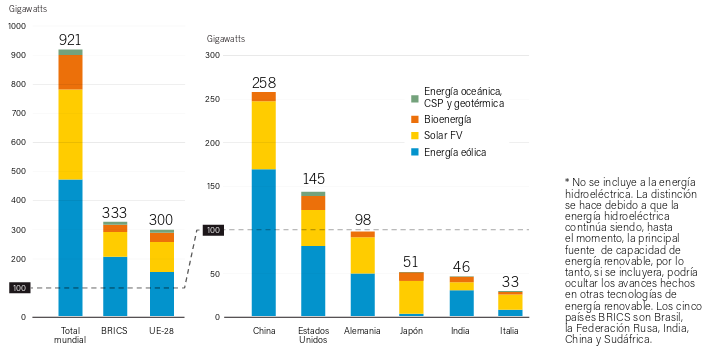
\includegraphics{/home/lewi/geaWaves/gea-waves/_hugo/content/tfg/1MEMORIA/imgMemoria/91-capacidadEERR.png}
\caption{}
\end{figure}

\textbf{Figura 9.1}: Capacidades de energía renovable* en el mundo,
EU-28, BRICS y los 6 países líderes, 2016.
\href{http://www.ren21.net/wp-content/uploads/2017/07/17-8399_GSR_2017_KEY-FINDINGS_Spanish_lowres.pdf}{Avanzando
en la transición mundial hacia la energía renovable}

La nueva capacidad de energía renovable instalada añadida marcaron un
nuevo record en 2016. Además, los costos disminuyeron de manera
vertiginosa, especialmente los relacionados a la energía solar FV y
eólica.

Ha habido un aumento importante en las ciudades, estados, naciones y
grandes corporaciones que se están comprometiendo a contar con objetivos
en materia de energía 100\% renovable porque, además de los beneficios
climáticos, ambientales y de salud pública, tiene más sentido en lo que
a negocios y economía se refiere. En 2016, 34 negocios se unieron a RE
100, que es una iniciativa mundial de empresas comprometidas a realizar
sus operaciones con electricidad 100\% renovable. Mientras que algunas
ciudades y comunidades han alcanzado este objetivo exitosamente
(incluyendo Burlington, Vermont en Estados Unidos y más de 100
comunidades en Japón).

Adicionalmente, desde REN21 se está planteando un cambio de paradigma en
los países en vías de desarrollo, en donde miles de millones de personas
aún no cuentan con acceso a la electricidad y/o instalacines limpias
para cocinar.

"\emph{El engorroso proceso de proporcionar acceso a la energía a través
de la red eléctrica se está volviendo obsoleto, pues existen modelos de
negocios y nuevas tecnologías que facilitan el desarrollo de mercados de
sistemas aislados}".

Los desarrollos realizados en torno a la energía renovable muestran que
el viejo paradigma de dotar acceso a la energía únicamente a través de
la extensión de la red eléctrica se está volviendo obsoleto. Para
acelerar el \textbf{acceso a la energía} es importante que la
legislación mire hacia el futuro, con el fin de que se pueda formar un
mercado estable, descentralizado y separado de la red, propiciando así
el desarrollo industrial.

Una gran número de políticas pueden ser útiles para acelerar este cambio
de paradigma:

\begin{itemize}
\item
  establecer objetivos específicos en materia de energía renovable
  distribuida a la par de objetivos en materia de electrificación y
  energía renovable que se implementen dentro de un cierto periodo de
  tiempo; 
\item
  integrar soluciones de sistemas autónomos a los planes nacionales de
  electrificación, en particular mini-redes; 
\item
  establecer un marco normativo claro para tener acceso a finanzas que
  reflejen este nuevo enfoque; 
\item
  así como medidas para mantener los estándares de calidad.
\end{itemize}

El Reporte sobre el futuro de las energías renovables en el mundo:
\textbf{grandes debates sobre la energía 100\% renovable}, lanzado en
abril de 2017. Analiza las perspectivas de más de 110 reconocidos
expertos en energía de todo el mundo, quienes fueron entrevistados en el
transcurso de 2016. Cabe señalar que el reporte no predice el futuro,
sino que tiene por objetivo estimular el debate sobre las oportunidades
y desafíos de un futuro basado en energía 100\% renovable y, por
consecuencia, ayudar a una mejor toma de decisiones.

Acceso a los reportes: \url{www.ren21.net/GSR} y \url{www.ren21.net/GFR}

\subsubsection{9.1.2 Estrategia europea de desarrollo
sostenible}\label{header-n72}

La UE viene marcando pautas en materia de medio ambiente desde hace más
de 30 años. En 1972, se decidió en la Cumbre Europea de París, elaborar
el primer programa de actuación. Las primeras Directivas, se centraron
especialmente en la calidad del agua, los productos y sustancias
químicas y la contaminación del aire. El papel de la UE es apoyar y
coordinar los esfuerzos de los Estados miembros y comprobar que los
gobiernos cumplen los compromisos adquiridos.
\href{https://e-archivo.uc3m.es/bitstream/handle/10016/12153/PFC_Carlos_\%20Caballero_Santos.pdf?sequence=1}{Fuente:
PFC-C.Caballero Santos 2011}

\textbf{Desarrollo sostenible} se refiere al esfuerzo por garantizar que
el crecimiento económico se lleve de tal manera que pueda ser compatible
y viable en el futuro sin agotar los recursos o perjudicar a la
sociedad. Este principio quedó ya reflejado en la Cumbre de Río de
Janeiro de las Naciones Unidas de 1992 cuando se fijó el doble objetivo
de trasformar las pautas contaminantes de consumo de los países
industrializados y luchar contra la pobreza.

Ya desde 1996 a nivel europeo, e incluso a nivel mundial con el
Protocolo de Kioto en 1997, se han ido evolucionando las diferentes
estrategias para adaptar las energías a un modelo sostenible. Estos
diferentes decretos han ido marcando las metas a las que se debían
llegar a nivel global y también nacional.

Esta información, se va actualizando y se puede consultar en el
Ministerio de Agricultura y pesca, alimentación y medio ambiente del
Gobierno de España, en la sección del Cambio Climático, documentación y
normativa del
\href{http://www.mapama.gob.es/es/cambio-climatico/temas/comercio-de-derechos-de-emision/documentacion-y-normativa/}{Comercio
de derechos de emisión}.

La política energética de la UE
(\href{https://europa.eu/european-union/topics/energy_es}{Unión Europea
- Energía}) persigue tres objetivos principales: seguridad de
abastecimiento, competitividad y sostenibilidad. A finales de 2013 la
comisión puso en marcha un plan,
\href{ec.europa.eu/priorities/energy-union-and-climate_es}{Unión de la
Energía}, basado en la actual política energética de la UE. Parte del
trabajo preliminar ya se ha llevado a cabo, Europa tiene un
\href{https://ec.europa.eu/energy/en/topics/energy-strategy-and-energy-union/2030-energy-strategy}{marco
de actuación energético y climático para 2030} y una
\href{https://ec.europa.eu/energy/en/topics/energy-strategy/energy-security-strategy}{estrategia
de seguridad energética}.

Europa se fijó los objetivos de clima y energía para 2020, 2030 y 2050:

\begin{itemize}
\item
  Objetivos para 2020:

  \begin{itemize}
  \item
    reducir las emisiones de gases de efecto invernadero un
    \textbf{20\%}, como mínimo, respecto a los niveles de 1990;
  \item
    obtener un \textbf{20\%} de la energía a partir de fuentes
    renovables;
  \item
    mejorar la eficiencia energética en un \textbf{20\%}.
  \end{itemize}
\item
  Objetivos para 2030:

  \begin{itemize}
  \item
    reducción de las emisiones de gases de efecto invernadero en un
    \textbf{40\%};
  \item
    al menos el \textbf{27\%} de energías renovables;
  \item
    aumento de la eficiencia energética en un \textbf{27-30\%};
  \item
    \textbf{15\%} de interconexión eléctrica, es decir, el 15\% de la
    electricidad generada en la UE debe poder transportarse a otros
    Estados miembros.
  \end{itemize}
\item
  Objetivos para 2050:

  \begin{itemize}
  \item
    el \textbf{80-95\%} de reducción de las emisiones de gases de efecto
    invernadero respecto a los niveles de 1990. La
    \href{http://eur-lex.europa.eu/legal-content/ES/ALL/?uri=CELEX:52011DC0885}{Hoja
    de Ruta de la Energía para 2050} muestra el camino para alcanzar esa
    meta.
  \end{itemize}
\end{itemize}

Como se ha visto, el liderazgo de la Unión Europea no se centra
únicamente en el ámbito de la mitigación. Cuando la Comisión hizo
pública la Estrategia Europea de Adaptación al Cambio Climático, también
tenía como objetivo orientar las actuaciones de las regiones para
reforzar la capacidad de adaptación de los sectores más vulnerables (la
salud, los recursos marinos y costeros, las infraestructuras, la
biodiversidad y los ecosistemas, la agricultura y el turismo) y mejorar
su resiliencia. Las principales líneas de actuación marcadas para la
adaptación al cambio climático se orientan hacia su integración en la
normativa y en las políticas financieras, y de forma paralela, continuar
mejorando el conocimiento como base para la toma de decisiones.

\begin{figure}
\centering
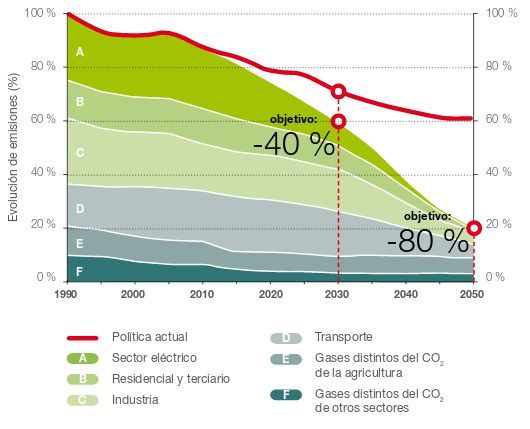
\includegraphics{/home/lewi/geaWaves/gea-waves/_hugo/content/tfg/1MEMORIA/imgMemoria/92-ruta2050UE.png}
\caption{}
\end{figure}

Figura 9.2: Hoja de ruta de la Unión Europea para la reducción de
emisiones a 2050. Fuente: Comisión Europea

\subsubsection{9.1.3 Estrategia nacional}\label{header-n130}

La Directiva 2009/28/CE del Parlamento europeo y del Consejo, relativa
al fomento del uso de energía procedente de fuentes renovables, fijó
como objetivo general conseguir un 20\% de energía procedente de fuentes
renovables en el consumo de la UE y un 10\% de energía renovable en el
sector del transporte para cada Estado miembro para el año 2020.

Así mismo, para junio de 2010 estableció la fecha límite para entregar
un Plan de Acción Nacional de Energías Renovables (PANER) para el
periodo 2011-2020, con vistas al cumplimiento de los objetivos
vinculantes que fija la Directiva. Hasta una semana antes de remitirlo a
la Comisión, estuvo abierto un proceso participativo para empresas,
asociaciones y ciudadanos, que realizaron aportaciones y sugerencias
para la elaboración del documento. El texto definitivo está a
disposición en la web de la Secretaría del Estado de Energía
\href{http://www.minetad.gob.es/energia/desarrollo/EnergiaRenovable/Paginas/paner.aspx}{PANER
2011-2020}, así como el anexo que contiene las normativas aplicables a
las energías renovables por Comunidad Autónoma.

\href{http://www.mapama.gob.es/es/cambio-climatico/temas/comercio-de-derechos-de-emision/el-comercio-de-derechos-de-emision-en-espana/}{El
comercio de derechos de emisión en España} de gases de efecto
invernadero está regulado por la Ley 1/2005, de 9 de marzo. Se puso en
marcha el 1 de enero de 2005, como medida fundamental para fomentar la
reducción de emisiones de \(CO_2\) en los sectores industriales y de
generación eléctrica.

Por otro lado, el otorgamiento del
\href{http://www.minetad.gob.es/energia/electricidad/energias-renovables/Paginas/renovables.aspx}{régimen
retributivo específico} se establecerá con carácter general mediante un
procedimiento de concurrencia competitiva, de acuerdo con lo dispuesto
en el
\href{http://www.boe.es/buscar/act.php?id=BOE-A-2013-13645\&tn=1\&p=20140328\&vd=\#a14}{artículo
14.7 de la Ley 24/2013, de 26 de diciembre}.

En el
\href{http://www.boe.es/diario_boe/txt.php?id=BOE-A-2014-3376}{Real
Decreto 216/2014}, de 28 de marzo, se establece la metodología de
cálculo de los precios voluntarios para el pequeño consumidor de energía
eléctrica y su régimen jurídico de contratación.

Mediante el
\href{https://www.boe.es/diario_boe/txt.php?id=BOE-A-2014-6123}{Real
Decreto 413/2014}, de 6 de junio, se regula la actividad de producción
de energía eléctrica a partir de fuentes de energía renovables,
cogeneración y residuos. La norma fundamental que ha regulado estos
aspectos ha sido la Ley 54/1997, del Sector Eléctrico. Durante los
últimos 20 años, junto con el desarrollo tecnológico para la producción
de energía eléctrica, se ha ido produciendo una simultánea evolución de
los marcos normativos de apoyo a fin de procurar su adaptación a las
circunstancias concurrentes en cada momento.

\href{http://www.boe.es/diario_boe/txt.php?id=BOE-A-2014-13475}{Orden
IET/2444/2014}, de 19 de diciembre, por la que se determinan los peajes
de acceso de energía eléctrica para 2015.

La normativa sobre
\href{http://www.minetad.gob.es/energia/electricidad/Tarifas/Paginas/index.aspx}{tarifas
eléctricas} que actualmente se encuentran en vigencia son:

\begin{itemize}
\item
  \href{https://www.boe.es/diario_boe/txt.php?id=BOE-A-2015-13782}{Orden
  IET/2735/2015}, de 17 de diciembre, por la que se establecen los
  peajes de acceso de energía eléctrica para 2016 y se aprueban
  determinadas instalaciones tipo y parámetros retributivos de
  instalaciones de producción de energía eléctrica a partir de fuentes
  de energía renovables, cogeneración y residuos.
\item
  \href{http://www.boe.es/diario_boe/txt.php?id=BOE-A-2014-13475}{Orden
  IET/2444/2014}, de 19 de diciembre, por la que se determinan los
  \textbf{peajes de acceso de energía} eléctrica para 2015 (BOE
  26/12/2014).
\item
  \href{https://www.boe.es/diario_boe/txt.php?id=BOE-A-2014-5173}{Resolución
  de 14 de mayo de 2014, de la Dirección General de Política Energética
  y Minas}, por la que se determina el \textbf{valor del término DIFp} a
  aplicar por los comercializadores de referencia en la facturación del
  consumo correspondiente al primer trimestre de 2014 a los consumidores
  a los que hubieran suministrado a los precios voluntarios para el
  pequeño consumidor.
\item
  \href{http://www.boe.es/diario_boe/txt.php?id=BOE-A-2014-3376}{Real
  Decreto 216/2014}, de 28 de marzo, por el que se establece la
  metodología de cálculo de los \textbf{precios voluntarios} para el
  pequeño consumidor de energía eléctrica y su régimen jurídico de
  contratación.
\item
  \href{http://www.boe.es/diario_boe/txt.php?id=BOE-A-2014-1053}{Resolución
  de 31 de enero de 2014, de la Dirección General de Política Energética
  y Minas} , por la que se revisa el \textbf{coste de producción de
  energía eléctrica y los precios voluntarios} para el pequeño
  consumidor (BOE 01/02/2014).
\end{itemize}

Según el informe de REE (Red Eléctrica de España)
\href{http://www.ree.es/es/estadisticas-del-sistema-electrico-espanol/informe-de-energias-renovables}{Energía
Renovable en 2016}, las renovables representaron más del 45\% de la
potencia instalada y casi el 39\% de la generación nacional. En el
sistema peninsular, que supone cerla del 95\% de la generación nacional,
la cuota de renovables alcanzó casi un 41\%.

\begin{figure}
\centering
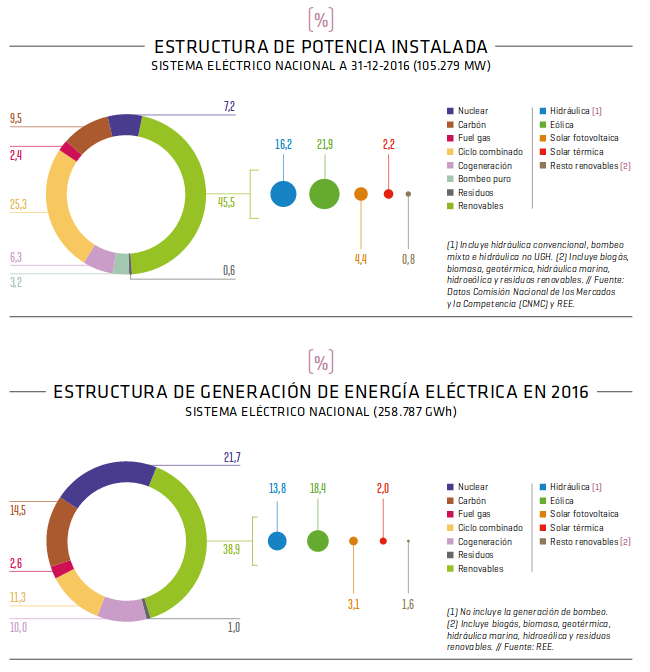
\includegraphics{/home/lewi/geaWaves/gea-waves/_hugo/content/tfg/1MEMORIA/imgMemoria/93-ree_skemaPotencial.png}
\caption{}
\end{figure}

Figura 9.3: Potencia instalada y generada a nivel nacional. {[}Fuente:
Informe de REE,
\href{http://www.ree.es/es/estadisticas-del-sistema-electrico-espanol/informe-de-energias-renovables}{Energía
Renovable en 2016}{]}

Como se muestra en la siguiente gráfica, a lo largo de los últimos 10
años las tecnologías eólica y solar son las que más crecimiento han
tenido.

\begin{figure}
\centering
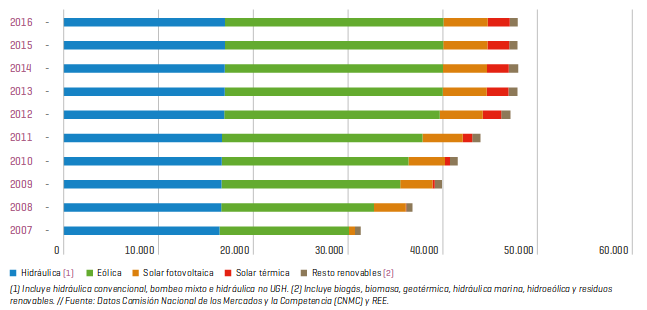
\includegraphics{/home/lewi/geaWaves/gea-waves/_hugo/content/tfg/1MEMORIA/imgMemoria/94-ree_evoluPotencial.png}
\caption{}
\end{figure}

Figura 9.4: Evolución del potencial instalado. {[}Fuente: Informe de
REE,
\href{http://www.ree.es/es/estadisticas-del-sistema-electrico-espanol/informe-de-energias-renovables}{Energía
Renovable en 2016}{]}

\subsubsection{9.1.4 Estrategia de cambio climático 2050 del País
Vasco}\label{header-n177}

La estrategia es el instrumento que permitirá consolidar una ciudadanía
comprometida con una economía sostenible y competitiva. Tal y como se
recoge en el documento
\href{http://www.euskadi.eus/contenidos/documentacion/klima2050/es_def/adjuntos/KLIMA2050_es.pdf}{KLIMA
2050}, la visión de Euskadi al año 2050 está asentada sobre cinco
premisas, cuya aplicación permitirá alcanzar los objetivos marcados:

\begin{enumerate}
\def\labelenumi{\arabic{enumi}.}
\item
  \textbf{Acción transversal}: Integrar la mitigación y adaptación al
  cambio climático en la planificación pública.
\item
  \textbf{Administración ejemplar}: Impulsar la acción ejemplarizante y
  coordinada de la Administración para lograr la transformación hacia
  una sociedad baja en carbono y adaptada.
\item
  \textbf{Innovación y oportunidades}: Apoyar la innovación y el
  desarrollo tecnológico, que permitan la reducción de emisiones de GEI
  en todos los sectores y reducir la vulnerabilidad del territorio al
  cambio climático.
\item
  \textbf{Cultura cero emisiones}: Favorecer la corresponsabilidad de
  todos los agentes de la sociedad vasca en las acciones de mitigación y
  de adaptación.
\item
  \textbf{Saber para transformar}: Adaptar el conocimiento local sobre
  cambio climático a la toma de decisión.
\end{enumerate}

Euskadi se ha fijado al año 2050 el objetivo de alcanzar un consumo de
energía renovable del 40\% sobre el consumo final. Así como reducir las
emisiones de GEI de Euskadi en al menos un 40\% a 2030 y en al menos un
80 \% a 2050, respecto al año 2005. Adicionalmente, en el mismo proyecto
vienen descritas las metas de cambio climático y las líneas de actuación
en euskadi.d

\begin{figure}
\centering
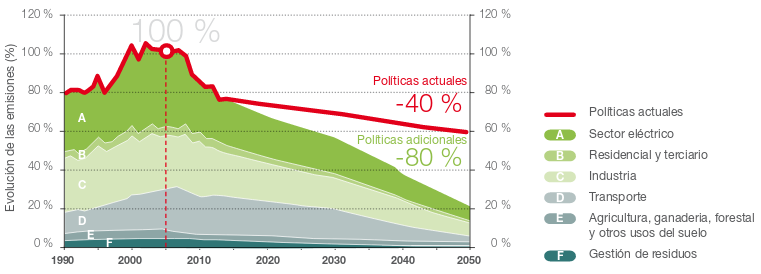
\includegraphics{/home/lewi/geaWaves/gea-waves/_hugo/content/tfg/1MEMORIA/imgMemoria/95-ruta-euskadi.png}
\caption{}
\end{figure}

Figura 9.5: Representación de la hoja de ruta de la Estrategia de Cambio
Climático del País Vasco 2050

\subsection{Costes}\label{header-n204}

El coste de la energía undimotriz depende de muchos factores, entre
ellos el coste capital y el coste de operación y mantenimiento. La
cantidad de energía producida vendrá relacionada con el coste, ya que si
un dispositivo trabaja proporcionando gran cantidad de energía, el coste
ponderado será menor que en uno cuya eficiencia es escasa. El balance
entre lo que supone económicamente producir y la cantidad que al final
se obtiene determinará el coste de la energía y si su explotación es
viable desde el punto de vista económico.

Es evidente, que dichos valores dependerán fuertemente de la
localización y tamaño de la instalación, y que además irán variando año
tras año.

El \textbf{coste capital} viene definido por cinco puntos:

\begin{itemize}
\item
  Coste de proyecto, incluyendo el dispositivo, cableado submarino,
  transporte de la energía y conexión. 
\item
  Coste de la estructura, es decir, de los materiales, componentes,
  procesos, y todo aquello relacionado con el dispositivo en si mismo y
  el sistema de conversión de energía. 
\item
  El coste de instalación del dispositivo. Cabe señalar que tanto los
  estudios terrestres como las obras civiles y de montaje, para las
  tecnologías undimotrices generalmente son menores, sobre todo, cuando
  son estructuras flotantes, debido a que sólo se deben instalar las
  líneas de amarre. 
\item
  Coste de la cimentación y amarres. El cual, supone un porcentaje
  importante dentro del coste capital, por ello no se incluye en el
  coste de la estructura. 
\item
  Coste de conexión a la red local. Varía en el caso de dispositivos
  onshore, nearshore o offshore, siendo éstos últimos los más costosos. 
\end{itemize}

Es importante destacar que el coste capital no es estático sino que va
evolucionando a lo largo del tiempo. A medida que surgen mejoras
tecnológicas y se gana experiencia, varían los precios de materiales,
evoluciona el coste de otras energías y se construyen mayor número de
dispositivos, reduciendo el coste capital. Sin embargo, hoy en día la
inmadurez técnica, el riesgo asociado a ésta tecnología, la falta de
economías de escala y la gran inversión inicial requerida, hacen que el
coste capital sea elevado pero con expectativas de disminuir.

Para poder comparar diferentes dispositivos, es frecuente distinguir
entre grandes grupos que en su conjunto formen el coste capital.

Debido a la falta de proyectos comerciales instalados en la actualidad
para la mayoría de las tecnologías, es difícil conocer los
\textbf{costos asociados a la instalación} del parque, por lo que,
amenudo, se estiman en base al costo de inversión.

\textbf{Indicadores de costes}: En ocasiones se utiliza el valor del
coste total por unidad de potencia instalada para, así, normalizar el
valor del coste y poder compararlo con otras tecnologías o para estimar
el coste en caso de querer cambiar la potencia instalada.

\textbf{Indicador ambiental}: Es posible construir un índice que
caracterice a las tecnologías por su impacto al ambiente en base a los
potenciales impactos. No obstante, si se consideran otros tipos, se
pueden llegar a otras conclusiones, luego no es posible considerarlo
como un indicador permanente.

\textbf{Coste de operación y mantenimiento}: Estos costes se deben
incluir anualmente, dependerán del tipo de tecnología, teniendo que
particularizarse para cada caso los riesgos que pudieran darse. En
general, la tecnologia unimotriz, al estar en constante movimiento y
expuesto a las condiciones variables del mar, deben analizarse estos
riesgos con especial cuidado.

\subsection{Novedades destacables}\label{header-n241}

\begin{itemize}
\item
  \href{http://www.agenergia.org/index.php?section=20}{Agencia Insular
  de Energía de Tenerife}

  En una región aislada geográficamente, como Tenerife, lograr una mayor
  diversificación energética resulta imprescindible, al disponer de
  recursos energéticos propios muy limitados y de una alta dependencia
  energética del exterior.

  En este contexto, la Agencia Insular de Energía de Tenerife trabaja
  con el objetivo de aunar los esfuerzos de todos los agentes implicados
  para la racionalización del consumo energético de Tenerife y para
  lograr una mayor diversificación de fuentes energéticas.

  Para ello, encargaron un proyecto "Plan de desarrollo regional para el
  uso de la energía proveniente del oleaje atlántico" \textbf{Proyecto
  Wave Energy}, publicado en 2007 por el Instituto Tecnológico y de
  Energías Renovables, SA (ITER, SA) con la participación de la UE y
  cofinanciado por el FEDER. El proyecto que consta de las siguientes
  acciones

  \begin{itemize}
  \item
    \href{http://www.agenergia.org/index.php?action=view\&id=53\&module=resourcesmodule\&src=\%40random49140d138ac53}{Estudio
    Comparativo de las diferentes fuentes de energía renovable marina}
  \item
    \href{http://www.agenergia.org/index.php?action=view\&id=54\&module=resourcesmodule\&src=\%40random49140d138ac53}{Estudio
    del estado del arte en cuanto a sistemas de generación undimotriz
    existentes}
  \item
    \href{http://www.agenergia.org/index.php?action=view\&id=276\&module=resourcesmodule\&src=\%40random49140d138ac53}{Informe
    sobre Corrientes Marinas - AIET}
  \item
    \href{http://www.agenergia.org/index.php?action=view\&id=56\&module=resourcesmodule\&src=\%40random49140d138ac53}{Presentación
    "La Energía del Océano" - ITER - Proyecto Wavenergy}
  \end{itemize}

  En 2014, se puso en marcha un sistema de energía undimotriz en Gran
  Canaria, financiado por el Ministerio de Economía y Competitividad a
  través del programa INNPACTO 2011 y, también, con fondos FEDER de la
  Unión Europea. Como se ha mencionado, el principal impedimento para
  esta fuente de energía es la financiación, aunque gracias a pasos como
  éste, se podrá alcanzar el aprovechamiento de los recursos que brinda
  la naturaleza y así minimizar nuestra huella ambiental.
  \href{https://www.solucionesintegralesendesa.com/blog/equipamiento-hogar/ahorro-hogar/energia-undimotriz-el-poder-de-las-olas/}{Blog
  SI - soluciones integrales}
\item
  Asociación de Energía Renovable Portuguesa (APERN)

  Según los datos de REN (Redes Energéticas Nacionais) Portugal generó
  en marzo más electricidad de origen renovable (4.812 GWh) que su
  consumo total (4.647 GWh). Unas cifras que se traducen en que
  \textbf{en términos netos las energías renovables generaron el 103,6\%
  de la demanda eléctrica}. Es decir, a pesar de haber tenido periodos
  en los cuales se ha necesitado de las centrales térmicas o importacon
  para abstecer la demanda eléctrica; en otros, la generación renovable
  ha estado por encima de la demanda.

  Los datos de generación más destacados fueron, publicados en
  \href{https://www.diariorenovables.com/2018/04/portugal-genero-100-electricidad-energias-renovables.html}{diario
  renovables}: las renovables registraron \textbf{un valor mínimo de
  cobertura del 86\%}, ocurrido el 7 de marzo, y \textbf{un máximo del
  143\%}, el 11 de marzo. Además, durante el periodo de 70 horas (desde
  el día 9) y de 69 horas (empezando desde el día 12) el consumo se
  abasteció por completo con fuentes renovables. 
\item
  Instituto Costarricense de Electricidad

  A lo largo de los primeros 75 días del año 2015, según el Instituto
  Costarricense de Electricidad fue innecesario el uso de hidrocarburos
  para alimentar la red del país. Una de las claves fue integrarse en el
  Programa de Energías Renovables y Eficiencia Energética de
  Centroamérica, implementado por la oficina para la Cooperación
  Internacional del Gobierno de Alemania, junto a la Secretaría General
  del Sistema de Integración Centroamericana (SG-SICA), que trabajan por
  fomentar una energía limpia en la región.

  Tabaré Arroyo, autor del estudio "Líderes en Energía Limpia" producido
  para la organización ambientalista World Wild Fund (WWF) destaca que
  el país centroamericano no solo invierte en energía hidroeléctrica,
  sino también en eólica y geotérmica, publicado por
  \href{http://www.bbc.com/mundo/noticias/2015/03/150323_costa_rica_energia_renovable_az_ep}{BBC
  Mundo}.

  En su informe para WWF, Arroyo califica a Costa Rica como "un líder
  regional en la implementación de políticas a favor de las energías
  renovables", siendo dos, los principales mecanismos establecidos para
  facilitar la inclusión de las renovables.:

  \begin{enumerate}
  \def\labelenumi{\arabic{enumi}.}
  \item
    Un "sistema específico de subastas por tecnología" que permitió
    incrementar la contratación de capacidad adicional.
  \item
    Un programa para "fomentar la generación local a manos de
    consumidores, quienes pueden vender exceso de energía a la red".
  \end{enumerate}

  Gracias a esto, Costa Rica creó un atractivo ambiente para las
  inversiones en energía renovable, señala el documento de WWF. Entre
  2006 y 2013, atrajo más de 1,700 millones de dólares para financiación
  de proyectos de energías renovables. En 2013, se alcanzó la cifra de
  600 millones de dólares americanos invertidos en energías renovables.

  En 2015, produjo el 98,95\% de su electricidad con energías
  renovables, publicado en
  \href{https://www.univision.com/noticias/energias-renovables/costa-rica-ha-producido-el-99-de-su-electricidad-con-renovables-en-2015}{uni
  vision noticias}, como especificó Carlos Obregón Quesada, presidente
  ejecutivo del ICE, el reparto exacto de la producción fue la
  siguiente: energía hidroeléctrica (75,53\%), geotérmica (12,88\%),
  eólica (9,81\%), biomasa (0,72\%), solar (0,01\%) y combustibles
  fósiles (1,05\%).

  Desde mayo del 2016, el 100\% de la energía en Costa Rica es de
  fuentes renovables. Según el presidente ejecutivo del ICE, la
  expectativa es concluir el año con al menos un 98\% de generación
  eléctrica a partir de fuentes renovables. {[}Fuente:
  \href{http://www.elespectador.com/noticias/medio-ambiente/mayo-el-100-de-energia-costa-rica-de-fuentes-renovables-articulo-647158}{el
  espectador noticias}{]}
\item
  Oceantec Marmok

  Respecto a la tecnología desarrollada en la actualidad, a modo de
  ejemplo, se pueden destacar las pricipales ventajas del convertidor de
  \href{http://www.oceantecenergy.com/desarrollo-tecnologico/}{Oceantec},
  explicado con más detalle en la sección de \href{}{6. Análisis de
  Alternativas}:

  \begin{itemize}
  \item
    Supervivencia: Las boyas cilíndricas han demostrado su supervivencia
    por muchos años. Hay boyas de navegación con formas similares que
    han estado sometidas casi 100 años a las condiciones de mar abierto.
  \item
    Bajo coste de mantenimiento asociado a su simplicidad: El
    convertidor de OCEANTEC tan solo tiene una parte móvil, la turbina,
    que es fácilmente accesible para trabajos de mantenimiento. Este
    hecho incrementa drásticamente la confiabilidad y reduce el coste de
    mantenimiento en comparación con otras tecnologías de captación de
    energía de las olas.
  \item
    Coste de la energía: Tras un análisis conceptual de diferentes
    tecnologías podemos asegurar que esta tecnología ofrece los menores
    costes de energía para obtener energía de las olas.
  \end{itemize}
\end{itemize}
